\documentclass[11pt,a4paper]{article}
\usepackage{ls}
\usepackage[german]{babel}

\title{Handreichung für die Seminararbeiten\\ im Modul \emph{Angewandte
    Informatik}\\ im Wintersemester 2020/21}

\author{Hans-Gert Gr\"abe}

\date{28. Januar 2021}

\begin{document}
\maketitle

\section{Hintergrund}

Im Bereich der TRIZ-Forschung wurde vor einem Jahr das \emph{TRIZ Summit
  Ontologie-Projekt}\footnote{Siehe \url{https://triz-summit.ru/onto_triz/}
  (in Russisch).}  begonnen, um die verschiedenen Teile der TRIZ-Theorie
ontologisch zu „kartieren“ und die wesentlichen Zusammenhänge zwischen den
einzelnen Teilen mit Mitteln semantischer Technologien zu erfassen. Hierzu
liegen aktuell vor
\begin{itemize}[noitemsep]
\item[(1)] eine „Übersichtskarte“ der verschiedenen Theoriefelder und der
  Zusammenhänge zwischen diesen,
\item[(2)] ein „Atlas“ von Ontokarten, die grob einzelne Bereiche markieren,
  die weiter zu detaillieren sind,
\item[(3)] zu einzelnen dieser Ontokarten erste Versuche, Struktur in das
  begriff\-liche Chaos zu bringen,
\item[(4)] ein Glossar (oder auch nur ein Thesaurus) von Begriffen, die
  hierfür wichtig sind.
\end{itemize}

Während zu (1) und (2) weitgehend Konsens besteht, sind die Modellierungen in
(3) stark umstritten, da die entsprechenden Semantiken und Zusammenhänge in
den unterschiedlichen TRIZ-Schulen naturgemäß unterschiedlich verstanden
werden.

Streit gibt es auch zu (4), der aber deutlich einfacher zu klären ist, wenn 
\begin{itemize}[noitemsep]
\item[(4a)] zunächst einmal alle Begriffe gesammelt und „URIfiziert“ werden
  (Thesaurus raw),
\item[(4b)] URIs so weit zusammengeführt werden, dass verschiedene URIs auf
  verschiedene Konzepte verweisen, aber Raum bleibt, für gleiche Konzepte
  verschiedene Semantiken zu hinterlegen (Thesaurus final),
\item[(4c)] diese verschiedenen Semantiken auch wirklich zusammengetragen und
  formalisiert werden (Glossar raw) und schließlich
\item[(4d)] die Semantiken in einem komplexen sozialen Abstimmungsprozess so
  weit wie \emph{möglich} abgeglichen und essenzielle Differenzen semantisch
  modelliert werden. 
\end{itemize}
In \cite{Kuryan2019} wird das Projekt genauer beschrieben, in
\cite{Kuryan2020} der aktuelle Stand dargestellt. Andere Vorarbeiten fanden
wenig Berücksichtigung\footnote{Details dazu auf der Webseite
  \url{https://wumm-project.github.io/Ontology.html}.}, insbesondere weder
\cite{IDM2011} noch \cite{GSA} oder \cite{VDI}. Im Herbst 2020 lief eine
Webinarreihe (in Russisch), deren Materialien auch verfügbar\footnote{Siehe
  \url{https://wumm-project.github.io/OntologyWebinar}.} und teilweise ins
Englische übersetzt sind.

Arbeitsgrundlage der TRIZ Summit Ontologie-Projekts ist ein Glossar von
V. Souchkov \cite{SG}, wobei dessen Einträge sowohl drei TRIZ-Generationen
(TRIZ-1..3) als auch 5 Kategorien (Basisbegriffe, Modelle, Regeln,
Begriffsgruppen, Synonyme) zugeordnet werden. Ein Webinarteilnehmer wies auf
einen weiteren Thesaurus \cite{GSA} auf den einschlägigen russischen
Altschullerseiten hin, der bereits multilingual vorliegt.

Im Rahmen des WUMM-Projekts wurden und werden Teile dieser Ontologisierungen
nachmodelliert und im \emph{WUMM RDFData github Repo}\footnote{Siehe dazu das
  Verzeichnis \texttt{Ontologies} im github-Repo
  \url{https://github.com/wumm-project/RDFData}} hochgeladen, die im Original
bisher ausschließlich durch grafische Ontogramme sowie die Möglichkeit einer
visuellen Inspektion im verwendeten OSA-Ontologie-Editor\footnote{Siehe
  \url{https://onto.devtas.ru/ts2o1} (in Russisch).} zugänglich sind.  Diese
im Original ausschließlich russischsprachigen Quellen wurden dabei in Teilen
auch ins Englische und Deutsche übertragen.  Weitgehend semantisch erfasst
sind (1) und (2). Weiterhin wurde bereits früher das VDI-Glossar „RDFiziert“
und die dort vorhandenen deutschen und englischen Erläuterungen um eine
russische Übersetzung ergänzt. Dies sowie der einfach zu transformierende
Thesaurus auf den Altschullerseiten bilden die Grundlage für einen eigenen
Thesaurus nach (4a), der mit den Begriff\-lichkeiten des Originalprojekts
weiter abzugleichen ist.  Inzwischen wurde auch das Glossar \cite{SG} in der
aktuellen Version 1.2 auf diese Weise aufbereitet.  Details dazu weiter unten.

\section{Themen für Seminararbeiten}

In den Seminararbeiten soll am Punkt (3) weitergearbeitet werden, indem für
eine konkrete Ontokarte $X$ (bzw. einen anderen konkreten
Modellierungszusammenhang im TRIZ-Kontext entsprechend den mündlichen
Absprachen)
\begin{itemize}[noitemsep]
\item[(A)] die Zusammenhänge für das WUMM-Projekt in RDF in einer gemeinsamen
  Rahmensetzung nachmodelliert werden sowie
\item[(B)] differierende Semantiken, Probleme und Widersprüche im Verständnis
  der modellierten TRIZ-Konzepte zusammengetragen und systematisiert werden.  
\end{itemize}
Während (A) primär einen ingenieur-technischen Charakter hat, erfordert (B)
stärker einen akademischen Zugang von Recherche und Vergleich einschlägiger
Publikationen.

Informationen zu (A) liegen typischerweise in Form von RDF-Diagrammen vor, wie
etwa die \emph{Top Level Ontologie} in Abbildung 1, und sollen in eine
Turtle-Datei vergleichbar zur Datei \texttt{TopLevel.ttl} im WUMM RDFData
github Repo überführt werden. 

\begin{center}
  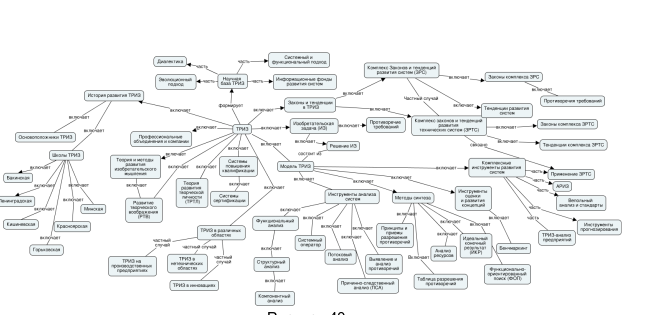
\includegraphics[width=\textwidth]{3.png}\\
  \textbf{Abbildung 1:} Die Top Level Ontologie als RDF Graph
\end{center}

Entsprechende Quellen für einen Startpunkt Ihrer Recherchen finden Sie in der
README-Datei in Ihrem Projektverzeichnis.

Für jede Seminararbeit ist ein Unterverzeichnis eingerichtet. Bitte forken Sie
(so weit noch nicht geschehen) das Repo auf einen eigenen Account, erstellen
die Seminararbeit und geben Zwischen- und das Endergebnis über einen
Merge-Request zur Begutachtung frei. Ich werde mich bemühen, die Ergebnisse
kurzfristig zu durchzusehen und mit Ihnen zu besprechen.

Die Seminararbeit selbst soll in {\LaTeX} erstellt werden und möglichst in
Englisch verfasst sein.

\section{Grundlagen des WUMM-Ontologie-Projekts}

Im TRIZ Summit Ontologie-Projekt geht es zunächst darum, die
TRIZ-Begriffslandschaft zu „kartieren“.  Das WUMM-Ontologie-Projekt begleitet
diese Aktivitäten, um
\begin{enumerate}[noitemsep]
\item eine Remodellierung nach semantischen Standards auszuführen,
\item die Materialien multilingual aufzubereitet und
\item auf dieser Basis eine LOD-Infrastruktur aufzubauen,
\end{enumerate}
und so eine bessere Basis für die erforderlichen sozialen Abstimmungsprozesse
zu schaffen.

\subsection{Die SKOS Ontologie als Basis}

Dafür wird die SKOS-Ontologie \cite{SKOS} verwendet, die mit den Konzepten (K)
\begin{itemize}[noitemsep]
\item \texttt{skos:Concept}, \texttt{skos:prefLabel}, \texttt{skos:altLabel}
  -- Objektbenennung
\item \texttt{skos:definition}, \texttt{skos:example}, \texttt{skos:note} --
  Objekteigenschaften
\item \texttt{skos:narrower}, \texttt{skos:broader} -- Objektrelationen
\end{itemize}
einen ersten Beschreibungsrahmen für Begrifflichkeiten bietet.  Für die
genauere Bedeutung der einzelnen Konzepte wird auf \cite{SKOS} verwiesen.  Auf
der Basis wurden bisher drei Quellen ausgewertet,
\begin{itemize}[noitemsep]
\item der mehrsprachige Thesaurus \cite{GSA},
\item das Glossar der VDI-Norm \cite{VDI} und
\item das Glossar \cite{SG}, Version 1.2, von V. Souchkov.
\end{itemize}
Außerdem wurde das Glossar des TRIZ Summit Projekts teilweise integriert.
Deren Glossar ist derzeit öffentlich nur in einer HTML-Version verfügbar.
Interne maschinenlesbare Versionen wurden mit dem Verweis auf den vorläufigen
Charakter der Modellierung noch nicht zur Veröffentlichung freigegeben.  Auch
lassen sich Daten in der OSA-Plattform nicht ohne Weiteres über eine API in
gängigen RDF-Formaten extrahieren. Deshalb habe ich den genaueren Abgleich
zugunsten der Konsolidierung des WUMM-Thesaurus zurückgestellt.

\subsection{URIs und Namensräume}

Eines der zentralen Probleme der Überführung der vorhandenen Datenbestände zu
TRIZ-Konzepten ist die Zuweisung sinnvoller URIs, da die einzelnen
Glossareinträge in den bisherigen Quellen einzig durch ihre Bezeichner
(„labels“) identifiziert werden.  Hier macht auch die OSA-Plattform keine
Ausnahme, denn die dort vergebenen URIs (sowohl für die Knoten als auch die
Kanten des aufgebauten RDF-Graphen) sind nicht öffentlich sichtbar.

Bei der maschinellen Transformation der Datenbestände in ein valides
RDF-Format wurden für alle Konzepte automatisiert URIs erzeugt, die im
Namensraum \texttt{tc:} (wie \emph{TRIZ Concepts}) liegen. Eine wesentliche
noch bevorstehende Aufgabe ist die Unifizierung dieser URIs, also die
Zusammenführung von verschiedenen URIs, welche auf denselben Begriff
verweisen.  Diese Arbeit soll demnächst in Angriff genommen werden.

\subsection{Provenienz von Erläuterungen}

Ein weiteres Problem dieser ontologischen Modellierung ist die genauere
Darstellung der Provenienz der einzelnen Erläuterungen. Hierzu wurden die
unter (K) aufgeführten SKOS-Konzepte für jede einzelne Quelle durch Notationen
aus dem Namensraum \texttt{od:} verfeinert, um zunächst die „Welten“ der
einzelnen Autoren und TRIZ-Schulen separat zu erfassen.

\texttt{od:} ist der Namensraum, den das WUMM-Projekt verwendet, um dort seine
eigenen Konzepte zu entwickeln.  Eine genauere Beschreibung dieses Namensraums
in einer eigenen RDF-Datei steht noch aus, die durch die URIs repräsentierten
Konzepte sind bisher nur mündlich abgestimmt.

Entsprechende Notationsvariationen sind etwa
\begin{itemize}[noitemsep]
\item \texttt{skos:Concept} $\to$ \texttt{od:GSAThesaurusEntry},
  \texttt{od:VDIGlossaryEntry} \ldots
\item \texttt{skos:definition} $\to$ \texttt{od:SouchkovDefinition},
  \texttt{od:VDIGlossaryDefinition} \ldots
\item \texttt{skos:example} $\to$ \texttt{od:VDIGlossaryExample} \ldots
\end{itemize}
usw. Siehe dazu die RDF-Daten selbst, die über den SPARQL-Endpunkt
\begin{center}
  \url{http://wumm.uni-leipzig.de:8891/sparql}
\end{center}
des WUMM-Projekts durchsucht werden können.

Die \emph{Verwendung verschiedener Prädikatsbezeichner} erlaubt es, auf
einfache Weise die Herkunft -- etwa von Definitionen -- einzelnen Quellen
bereits auf der Ebene von Tripeln zuzuordnen:
\begin{center}
  (Begriff X) -- (wird in Quelle A definiert als) -- (Definition von X in
  Quelle A)\\ 
  (Begriff X) -- (wird in Quelle B definiert als) -- (Definition von X in
  Quelle B) 
\end{center}
Würde einheitlich \texttt{skos:definition} verwendet, so müssten komplexere
Konstrukte
\begin{center}
  (Begriff X) -- \texttt{skos:definition} -- \Big[\parbox{8cm}{\centering
      (Quelle A) -- (Definition von X in Quelle A)\\
      (Quelle B) -- (Definition von X in Quelle B)
    }\Big]
\end{center}
eingesetzt werden. Auch wenn dies das finale Ziel der Übung ist, soll im
aktuellen Stand der Modellierung die einfachere Form verwendet werden, obwohl
damit die Zahl der Prädikate aufgebläht wird. Eine Konsolidierung der
Modellierung in Richtung des „idealen Endresultats“ ist später durch eine
einfache Modelltransformation zu erreichen.

Dasselbe gilt für die Verwendung von provenienzabhängigen Unterklassen von
\texttt{skos:Concept}.  Da der Abgleich der für Konzepte vergebenen URIs
unterklassenübergreifend erfolgen muss, sind die Instanzen jeder Unterklasse
auch als \texttt{skos:Concept} ausgezeichnet, obwohl dies auch über einen
generalen Satz wie etwa
\begin{center}\tt
  od:VDIGlossaryEntry rdfs:subClassOf skos:Concept
\end{center}
beschrieben und dann durch Inferenz festgestellt werden könnte. Das Inferieren
von Eigenschaften gehört aber zu komplexeren semantischen OWL-Konzepten und
wird von einfachen RDF-Stores nicht unterstützt. Auch hier gilt, dass die
Daten später durch eine einfache Modelltransformation konsolidiert werden
können.

\subsection{Modellierung eines TRIZ-Teilgebiets}

Typischerweise liegt das zu modellierende Teilgebiet als RDF-Graph
vergleichbar zu Abbildung 1 vor.  Dazu ist eine eigene Turtle-Datei anzulegen
und zu befüllen, welche diesen Graphen nachmodelliert.

Die RDF-Modellierung eines solchen Graphen sollte in drei Schritten
vorgenommen werden:
\begin{enumerate}
\item Modelliere zunächst die Knoten als TRIZ-Konzepte, wobei möglichst URIs
  und damit Konzepte aus dem vereinten Glossar (also bereits vorhandene
  Instanzen vom Typ \texttt{skos:Concept}) verwendet werden sollten.  Die
  Knotenbeschriftung ist entweder schon im Glossar oder als
  \texttt{skos:prefLabel} oder (in einzelnen Fällen) als
  \texttt{skos:altLabel} (in Ihrer Datei) zu ergänzen, ggf. auch
  mehrsprachig. In jedem Fall muss das Label einen RDF-Sprachtag tragen.

  Wenn Sie neue Konzept-URIs einführen, müssen diese im Namensraum
  \texttt{tc:} liegen und als sowohl zum RDF-Typ \texttt{skos:Concept} als
  auch \texttt{od:AdditionalConcept} gehörend ausgezeichnet sein.
\item Modelliere danach die Kanten, wobei neue oder bereits vorhandene
  Prädikat-URIs aus dem Namensraum \texttt{od:} verwendet werden.  Die Wahl
  der URI sollte sich an einem kurzen englischen Begriff als „sprechender
  Name“ orientieren.

  Prädikate haben zunächst keinen Label, allerdings müssen Kanten im Graphen
  mit gleichem Label durch dieselbe Prädikat-URI modelliert werden.  Zur
  Auswahl von Prädikat-URIs unten mehr. 
\item Ergänze schließlich Definitionen, Erläuterungen und Beispiele zu den
  Knoten (so weit vorhanden), die als \texttt{skos:definition},
  \texttt{skos:node} und \texttt{skos:example} zu modellieren sind. Auch hier
  bitte konsequent RDF-Sprachtags einsetzen. Wenn Sie differierende
  Erläuterungen desselben Prädikats aus unterschiedlichen Quellen erfassen,
  dann spalten Sie das SKOS-Prädikat in verschiedene Unterprädikate aus dem
  Namensraum \texttt{od:} auf wie im Abschnitt 3.3 erläutert.
\end{enumerate}
Wenn Sie nicht genau wissen, wie eine Objektinformation an einen Knoten
angebunden werden soll, dann verwenden Sie das Prädikat
\texttt{rdfs:comment}.

Bitte beachten Sie, dass Literale in einfachen Quotes keine Zeilenumbrüche
enthalten dürfen und Quotes im Text durch $\backslash$ ausgezeichnet werden
müssen. Am einfachsten vermeiden Sie einfache Quotes innerhalb von Strings und
ersetzen diese durch German Quotes („...“) oder French Quotes («...» in der
russischen und deutschen Schreibweise oder »...« in der französi\-schen).  Die
entsprechenden Zeichen sind auf gängigen deutschen Tastaturen in der
Alt-Gr-Belegung verfügbar. 

Mehrzeilige Literale können durch Einschließen in Triple-Quotes erstellt
werden. Dann müssen Quotes im Text auch nicht ausgezeichnet werden.

\subsection{Modellieren von Prädikaten und UML-Diagramme}

Ein Prädikat wird in einem RDF-Graphen durch einen beschrifteten gerichteten
Pfeil zwischen zwei Knoten markiert.   Oft gibt es zu einem Prädikat auch ein
inverses Prädikat (etwa \texttt{org:memberOf} und \texttt{org:hasMember}), das
einem Pfeil in umgekehrter Richtung entspricht.

Bitte beachten Sie, dass die Pfeile in den OSA-Diagrammen des TRIZ Summit
Ontologie-Projekts willkürlich gerichtet sind, da im Modellierungs-Tool stets
\emph{beide} Prädikate (direktes und inverses) benannt werden können, die
Richtung der Pfeile im Diagramm willkürlich ist und in verschiedenen Ansichten
auch wechselt.  Das gilt nicht für Cmap\footnote{Cmap ist ein weiteres
  grafisches Modellierungstool, das im TRIZ Summit Ontologie-Projekt
  eingesetzt wurde.}-Diagramme wie in Abbildung 1.

In Arbeiten wie etwa \cite{IDM2011} werden \emph{UML-Diagramme} zur
Modellierung verwendet, siehe etwa \cite[Fig. 2]{IDM2011}. Neben (wenigen)
benannten Pfeilen werden dort UML-Konstrukte wie Unterklasse und Aggregation
zur Darstellung von Beziehungen zwischen Klassen verwendet sowie
Objekteigenschaften durch Klassenattribute modelliert.  Diese müssen alle
durch Prädikate vom Typ \texttt{rdf:Property} \cite{RDFS} modelliert werden,
da erst in höheren semantischen Konzepten wie OWL \cite{OWL} Verfeinerungen
wie \texttt{owl:ObjectProperty} zur Verfügung stehen.  Es gibt keine
etablierten Standards, wie relationale UML-Konstrukte nach RDF umgesetzt
werden, weshalb Sie hier frei in der Wahl von Prädikat-URIs (aus dem
Namensraum \texttt{od:}) sind, wenn Sie gleiche UML-Konstrukte auch gleich
benennen.  Bei Attributen ist die Sache einfach, da sowohl der
\texttt{rdfs:domain} (die Klasse, zu welcher das Attribut gehört) als auch das
Label des Attributs gegeben sind.  Allein der \texttt{rdfs:range} muss
gelegentlich genauer bestimmt werden, wenn er nicht \texttt{rdfs:Literal} ist.
Bitte orientieren Sie sich auch hier an der Umsetzung der Top Level Ontologie
in der Datei \texttt{TopLevel.ttl}, insbesondere an den dort bereits
verwendeten Prädikat-URIs.

\section{Werkzeuge}

Im Zuge des Seminars haben Sie gezeigt, dass Sie mit {\LaTeX} umgehen können.
Bitte verwenden Sie möglichst die Style-Vorlage \texttt{ls.sty} im Repo für
die grundsätzlichen Definitionen und ergänzen Sie dies lokal in Ihrer
\LaTeX-Präambel.  \texttt{ls.sty} kann etwa durch einen symbolischen Link in
Ihrem Arbeitsverzeichnis verfügbar gemacht werden.

Das Erstellen einer RDF-Ontologie bedarf keiner besonderen Werkzeuge, da eine
Turtle-Datei eine Textdatei ist und mit jedem Texteditor erzeugt und
bearbeitet werden kann, der plain text (!) liefert.  Für die Validierung und
Transformation solcher Dateien haben sich die \emph{Redland RDF Libraries}
\url{http://librdf.org} und dort besonders das Kommandozeilen-Tool
\texttt{rapper}\footnote{\url{http://librdf.org/raptor/rapper.html}.  In
  gängigen Linux-Distributionen kann das über die Paketverwaltung installiert
  werden. } bewährt.
Mit \texttt{rapper -gc (RDF-Datei)} kann damit die Syntax einer RDF-Datei
validiert, mit 
\begin{center}\tt
  rapper -g (Eingabedatei) -o (format)
\end{center}
eine Eingabedatei in ein anderes RDF-Format (turtle, ntriples) umgewandelt
oder im selben Format normalisiert (und formatiert) werden.  Die Ausgabe
erfolgt auf \texttt{stdout} und muss ggf. umgelenkt werden.

\begin{thebibliography}{xxx}
\bibitem{IDM2011} D. Cavallucci, F. Rousselot, C. Zanni (2011). An ontology
  for TRIZ. Proc. TRIZ Future Conference 2009. Procedia Engineering 9,
  251–260.\\  \url{https://doi.org/10.1016/j.proeng.2011.03.116}.
\bibitem{Kuryan2019} A. Kuryan, V. Souchkov, D. Kucharavy (2019). Towards
  ontology of TRIZ. TRIZ Developers Summit, Minsk 2019.
  \\ \url{https://wumm-project.github.io/Texts/Ontology-TDS2019-en.pdf}
\bibitem{Kuryan2020} A. Kuryan, M. Rubin, N. Shchedrin, O. Eckardt, N. Rubina.
  TRIZ Ontology. Current State and Perspectives. TRIZ Developers Summit 2020
  (in Russisch). Englische Übersetzung:
  \\ \url{https://wumm-project.github.io/Texts/Ontology-TDS2020-en.pdf}
\bibitem{SG} V. Souchkov. Glossary of TRIZ and TRIZ-related Terms. Mehrere
  Versionen seit 1991. Letzte Version 1.2 von 2014.
\bibitem{GSA} Thesaurus auf \texttt{altshuller.ru}.
  \url{https://www.altshuller.ru/thesaur/thesaur.asp}
\bibitem{VDI} VDI Richtlinie 4521. Erfinderisches Problemlösen mit TRIZ.\\
  Blatt 1: Grundlagen und Begriffe (April 2016).\\ Blatt 2: Zielbeschreibung,
  Problemdefinition und Lösungspriorisierung (April 2018).\\ Blatt 3:
  Lösungssuche (Juli 2020). 
\bibitem{OWL} W3C (2004). OWL Web Ontology Language Guide.\\
  \url{https://www.w3.org/TR/2004/REC-owl-guide-20040210}
\bibitem{SKOS} W3C (2008). SKOS Simple Knowledge Organization System RDF
  Schema.\\
  \url{https://www.w3.org/TR/2008/WD-skos-reference-20080829/skos.html}
\bibitem{RDFS} W3C (2014). RDF Schema 1.1.
  \url{https://www.w3.org/TR/rdf-schema}
\end{thebibliography}

\end{document}
